%  Typ dokumentu - článek, prezentace aj.
\documentclass[english]{article}

%  Nastaví vstupní a výstupní kódování znaků (encoding) a lokalizace
\usepackage[T1]{fontenc}
\usepackage[utf8]{inputenc}
\usepackage[english,czech]{babel}
\usepackage{icomma}

%  Formát papíru a odsazení od jeho okrajů
\usepackage[letterpaper]{geometry}
\geometry{verbose,tmargin=1.5cm,bmargin=2cm,lmargin=2cm,rmargin=2cm}

%  Umožňuje pracovat s grafikou
\usepackage{graphicx}
\usepackage{bigstrut}
\usepackage{epstopdf}

%  Automaticky odsadí i první paragraf v každé sekci
\usepackage{indentfirst}

%  Umožňuje rozdělovat obsah na více sloupců
\usepackage{multicol}
\usepackage{booktabs}
\usepackage{pgffor}

% physics
\newcommand{\unit}[1]{\ \mathrm{#1}}
\newcommand{\dd}{\mathrm{d}}
\newcommand{\ee}{\mathrm{e}}
\newcommand{\bb}[1]{\boldmath{}\textbf{$\mathrm{#1}$}\unboldmath{}}
%  Umožňuje používat hypertextové odkazy, nastavuje jejich barvu a
%  vlastnosti
\usepackage[unicode]{hyperref}
\hypersetup{
colorlinks=true, citecolor=blue, filecolor=blue, linkcolor=blue,
urlcolor=blue
}

%  Formátování stránek, empty = odstraní číslování
% \pagestyle{empty}

%  Řádkování
\linespread{1.2}

%  Lepší zobrazování matematiky (rozšíření sum o \limits atd.)
\everymath{\displaystyle}
\usepackage{amsmath, amsthm, amssymb}

% Umožní psát přes \mathbb{N/R/Q/..} množiny čísel
\usepackage{amssymb}

%  Velikost fontu matematických výrazů v dokumentu lze pro danou
% základního fontu dokumentu upravit pomocí:
% \DeclareMathSizes{X}{Y}{Z}{U} kde:
% X je velikost fontu v dokumentu, pro kterou se matematika upraví
% Y je standartní velikost fontu matematiky
% Z je velikost fontu zmenšených (vnořených výrazů)
% U je velikost fontu ještě více zmenšených (vnořených výrazů).
\DeclareMathSizes{10}{10.5}{9}{9}

%  Nastaví autora, název, datum, skupinu měření apod. (můj vlastní
% příkaz, umožní znovu-použití v dokumentu)
\newcommand{\Author}{David Roesel}
\newcommand{\Coauthor}{Tereza Schönfeldová}
\newcommand{\Institute}{FJFI ČVUT v Praze}
\newcommand{\Subject}{FYZIKÁLNÍ PRAKTIKUM II}
\newcommand{\Group}{7}
\newcommand{\Circle}{ZS 7}
\newcommand{\Title}{Úloha \#14(5)  \\Měření rychlosti světla}
\newcommand{\Date}{5.5.2014}

% Začátek dokumentu - Formátování na výstup
\begin{document}

% Interní proměnné, možno zobrazovat u prezentací, používají se při
% generování pomocí \titlepage apod.
\author{\Author}
\title{\Title}
\date{\Date}

%  Lokalizace některých názvů do češtiny
\renewcommand{\figurename}{Obr.}
\renewcommand{\tablename}{Tab.}
\renewcommand{\refname}{Reference}

% --- Hlavička dokumentu -----------------------------------------------

\setlength{\parindent}{0cm}
\begin{multicols}{2}
\textbf{\Subject \\
        \Institute \\[0.1cm]
%\large  \Title \\[0.5cm]
\Title \\[0.5cm]
}
\begin{tabular}{rlrl}
\large Datum měření: & \Date & \large Skupina: & \Group \\
\large Jméno: & \Author & \large Kroužek:  & \Circle\\
\large Spolupracovala: & \Coauthor &\large Klasifikace:\\
\end{tabular}

\begin{flushright}

\includegraphics[scale=0.28]{../../_meta/fjfi_standart.pdf}
\hspace{0.2cm}
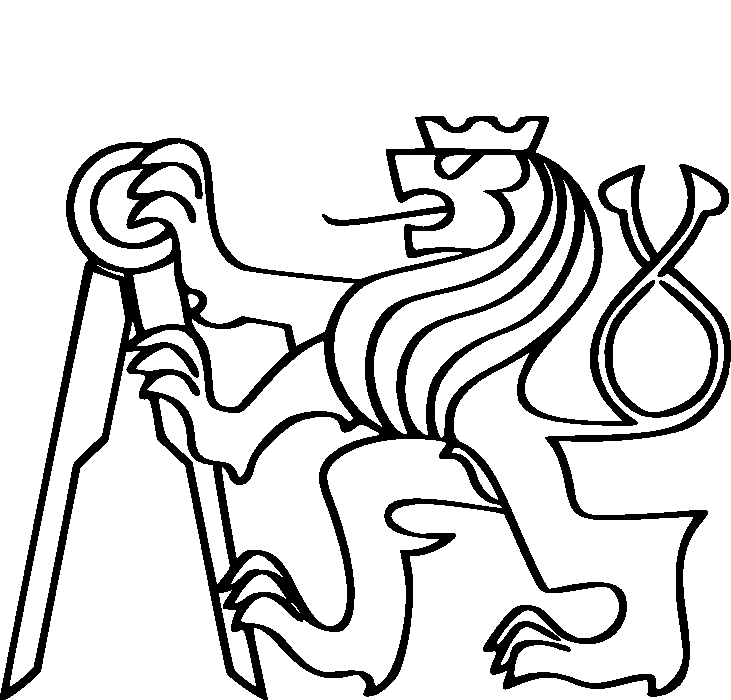
\includegraphics[scale=0.28]{../../_meta/cvut_standart.pdf}
\end{flushright}
\end{multicols}
\hrule
\vspace{0.5cm}

% ----------------------------------------------------------------------


% --- Tělo dokumentu ---------------------------------------------------
\setlength{\parindent}{0.5cm}
\section{Pracovní úkoly}
\begin{enumerate}
\item V domácí přípravě odvoďte vztah (1) z \cite{bib:zadani} včetně náčrtku.

\item V domácí přípravě odvoďte vztah pro střední odhad relativní chyby měření rychlosti světla $c$. Potřebné informace najdete na: 

\texttt{http://praktikum.fjfi.cvut.cz/documents/chybynav/CHYBY1n.pdf}

\item Vyberte si vhodné místo a předem si promyslete kam umístíte optickou lavici a kam pevné sférické zrcadlo. Poté sestavte (a nastavte) aparaturu dle návodu.

\item Vhodným způsobem změřte vzdálenosti $A$, $B$ a $D$ (viz Obr. \ref{fig:s_virtu}) a poznamenejte si chyby daných měření.

\item Proveďte měření alespoň pro 10 různých frekvencí v rozmezí 200~--~1300 ot./min. Vaše měření vhodným způsobem statisticky zpracujte.

\item Váš výsledek srovnejte s tabulkovou hodnotou $c$ a diskutujte.

\end{enumerate}

	
\section{Vypracování}

	\subsection{Použité přístroje}
		Modul s rotačním zrcátkem včetně ovládání, pevné sférické zrcadlo na podstavci, měřící mikroskop s děličem svazku, 2~čočky (ohniskové vzdálenosti 48~mm a 252~mm), polarizátor, 0,5mW He-Ne laser 632,8~nm, optická lavice 1~m spojená s nastavitelnou lavicí pro laser, zaměřovače svazku, mobilní telefon, výsuvné měřící pásmo, svinovací metr, nit.
			
	\subsection{Teoretický úvod}
			Náčrtek experimentu je znázorněn na Obr.~\ref{fig:s_fouc}. Laserové světlo prochází čočkou \bb{L_1} a je jí fokusováno do bodu \bb{s}. Následně prochází skrze polopopustné zrcadlo do čočky \bb{L_2}, která světlo fokusuje z bodu \bb{s} přes rotující zrcátko \bb{M_R} do bodu \bb{S} na sférickém zrcadle \bb{M_F} o pevné pozici. Ze sférického zrcadla \bb{M_F} se světlo odráží zpět na \bb{M_R} po původní dráze, ale rotující zrcátko zastihne v jiné poloze a tím pádem se obraz původního bodu \bb{s} zformuje do nového bodu \bb{s_1}. K pozorování tohoto obrazu je právě polopropustné zrcadlo mezi body \bb{L_1} a \bb{L_2}, které zobrazí bod \bb{s_1} do bodu \bb{s'}. 
			
				\begin{figure}[h!]
				\begin{center}
					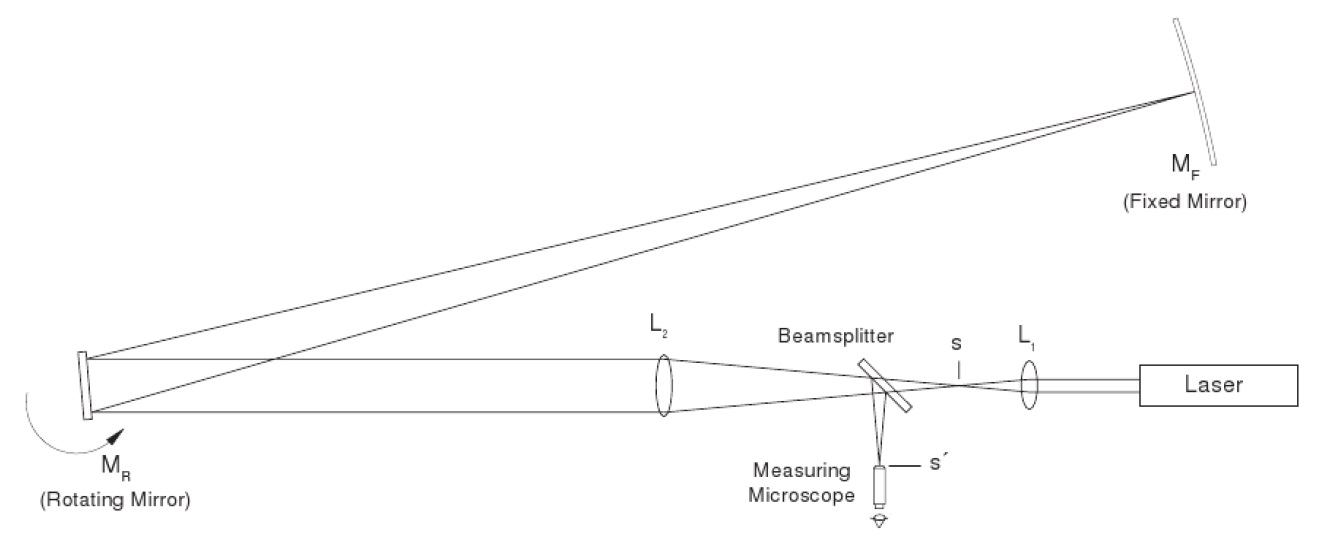
\includegraphics[width=\linewidth]{att/zakl_schema.jpg}
					\caption{Schéma experimentu - Foucaultova metoda. Převzato z \cite{bib:zadani}.}
					\label{fig:s_fouc}
				\end{center}
				\end{figure}
			
			Podrobný náčrtek dráhy, kterou světlo putuje, je znázorněn na Obr.~\ref{fig:s_draha}. Účelem tohoto sestavení je získat vztah mezi rychlostí světla a posunem bodu \bb{s\rightarrow s_1}, a je tak potřeba se detailně věnovat dráze, kterou bude světlo putovat. Poté co světlo projde čočkou \bb{L_2}, dopadne na rotační zrcadlo v momentu, kdy se nachází v první pozici (tedy pootočené o úhel $\theta$). Odrazí se směrem k \bb{M_F}, dopadne na něm do bodu \bb{S} a odrazí se zpět. Jeho dráha teď bude svírat úhel $2\theta$ s dráhou od laseru k \bb{M_R}. Při dopadu na \bb{M_R} je ale toto rotační zrcadlo ve druhé poloze vzhledem k otočení o úhel $\Delta\theta$. Paprsek světla se tím pádem odrazí směrem k laseru pod úhlem $2\Delta\theta$ od jeho spojnice s \bb{M_R}. 
			
			Představme si teď, že vracející paprsek dopadal na \bb{M_R}, když bylo v první poloze a ne ve druhé. To by znamenalo, že od \bb{M_F} vycházel ne z bodu \bb{S}, ale z nějakého nového bodu \bb{S_1}. Úhel mezi spojnicemi \bb{M_R} a \bb{S}/\bb{S_1} tím pádem bude $2\Delta\theta$. Pokud označíme vzdálenost \bb{M_R} a \bb{M_F} jako $D$, budou od sebe body \bb{S} a \bb{S_1} vzdáleny o $2D\Delta\theta$. 
			
				\begin{figure}[h!]
				\begin{center}
					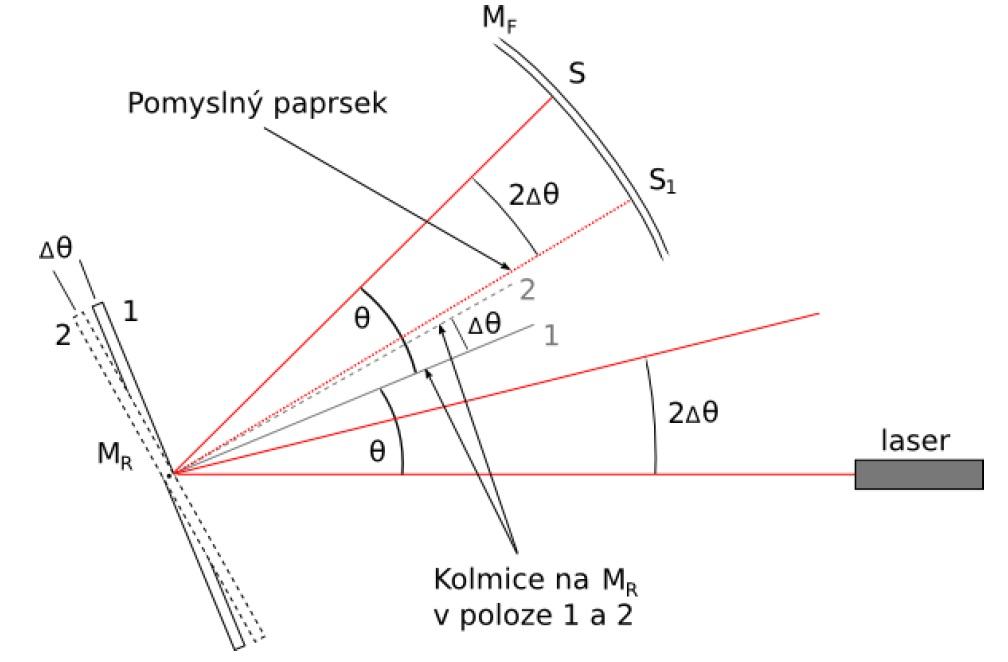
\includegraphics[width=0.7\linewidth]{att/draha_svetla.jpg}
					\caption{Schéma experimentu - náčrt pro odvození úhlů. Tečkovaná čára odpovídá dráze, po které by světlo putovalo, kdyby bylo zrcadlo při návratu světla z \bb{M_R} v poloze \bb{1} místo v poloze \bb{2}. Převzato z \cite{bib:zadani}.}
					\label{fig:s_draha}
				\end{center}
				\end{figure}			 
			
			Posun z \bb{s} do \bb{s_1} určíme jako vzdálenost $\Delta s = $ \bb{|s_1s|}, po odklonu polopropustným zrcadlem pak $\Delta s' = $ \bb{|s_1's'|}. Pro zpřehlednění použijeme nákres virtuálního obrazu \bb{M_F} na Obr.~\ref{fig:s_virtu}. Když je \bb{M_R} v první poloze, bude \bb{S} ležet přesně na ose svazku a bod \bb{S_1} od něj bude vzdálen o $\Delta S$. Tak jsme úlohu převedli na soustavu tenkých čoček.  
		
				\begin{figure}[h!]
				\begin{center}
					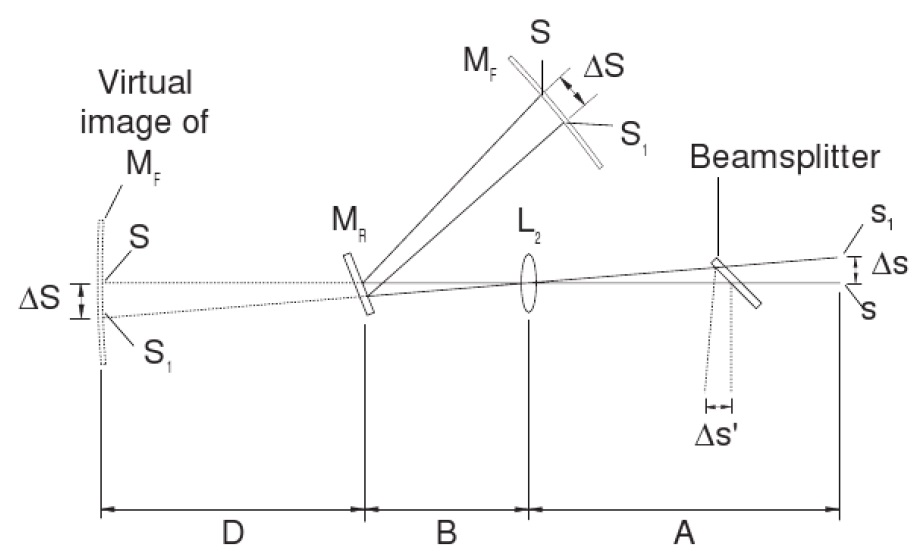
\includegraphics[width=0.7\linewidth]{att/virtu.jpg}
					\caption{Schéma experimentu - náčrt k analýze virtuálních odrazů. Převzato z \cite{bib:zadani}.}
					\label{fig:s_virtu}
				\end{center}
				\end{figure}			
				
			Pokud označíme vzdálenost mezi \bb{M_R} a \bb{L_2} jako $B=$\bb{|M_RL_2|} a vzdálenost mezi \bb{L_2} a \bb{s} jako $A=$\bb{|L_2s|}, bude platit vztah
			\begin{equation}
				\Delta s' = \Delta s = \frac{A}{D+B}\Delta S
			\end{equation}
			a pokud do něj dosadíme výše zmíněnou rovnost $\Delta S = 2D\Delta\theta$, získáváme
			\begin{equation}
				\Delta s' = \frac{2AD\Delta\theta}{D+B}.
			\end{equation}
			
			Velikost $\Delta\theta$ je závislá na tom, jak rychle se otáčí \bb{M_R}, a na době, jakou trvá světlu urazit vzdálenost $2D$. Úhel se tedy dá vyjádřit vztahem
			\begin{equation}
				\Delta\theta = \frac{4\pi D f}{c}.
			\end{equation}
			Dosadíme-li do sebe předchozí dva vztahy, získáme vztah pro rychlost světla, který můžeme zapsat ve tvaru
			\begin{equation}
				c = \frac{8\pi A D^2 f}{\left(D+B\right)\Delta s'}.
				\label{eq:c}
			\end{equation}
			K určení rychlosti světla tedy potřebujeme znát odpovídající vzdálenosti, vychýlení bodu $\Delta s'$ a frekvenci otáčení rotujícího zrcadla \bb{M_R}. Při našem měření budeme otáčet zrcátkem ve dvou různých směrech a proto tento vzorec lehce pozměníme do finálního tvaru
			\begin{equation}
				c = \frac{8\pi A D^2 \left(f_{CW}+f_{CCW}\right)}{\left(D+B\right)\left(s'_{CW}-s'_{CCW}\right)},
				\label{eq:ccw}
			\end{equation}
			kde $f_{cw}$ a $f_{ccw}$ jsou frekvence otáčení v obou směrech a $s'_{cw}$ a $s'_{ccw}$ odpovídající polohy bodu \bb{s'}.
			
	\subsection{Postup měření}
		Hlavní částí experimentu bylo sestavení aparatury, které jsme provedli podle nákresů v zadání úlohy \cite{bib:zadani}. Při práci s laserem jsme si dávali pozor, abychom se očima nepřiblížili horizontální rovině laseru. Ochranné brýle bohužel nebyly u úlohy k dispozici, bylo by je však v opačném případě moudré používat. Optická lavice již byla umístěna na rozhraní dvou stolů a na ní bylo správně připevněno rotační zrcátko \bb{M_R}. Dále jsme postupovali podle následujícího postupu.
		\begin{itemize}
			\item Umístíme laser na kratší část lavice.
			\item Pomocí zaměřovačů svazku nastavíme paprsek do středu \bb{M_R}.
			\item Odstraníme zaměřovač bližší k \bb{M_R} a zkontrolujeme vertikální zarovnání paprsku.
			\item Umístíme čočku \bb{L_1} na optickou lavici do vzdálenosti $93,0\unit{cm}$ od kraje s \bb{M_R}.
			\item Jemným pohybem čočky (ne podstavce) zarovnáme znovu paprsek do středu \bb{M_R}.
			\item Na lavici umístíme čočku \bb{L_2} do vzdálenosti $62,2\unit{cm}$ a znovu nastavíme paprsek do středu \bb{M_R}.
			\item Mezi čočky \bb{L_{1,2}} umístíme mikroskop s polopropustným zrcátkem (ale zatím se do něj nekoukáme).
			\item Pokud chceme koukat do mikroskopu, když nerotuje \bb{M_R}, umístíme mezi čočku \bb{L_2} a laser otočný polarizátor natočený na zhruba $89^\circ$ tak, aby blokoval většinu světla.
			\item Umístíme sférické zrcadlo, co nejdále to jde (na konec místnosti) a ujistíme se, že mezi ním a \bb{M_R} nic nepřekáží.
			\item S odebraným polarizátorem natočíme ručně (po odebrání pojistky) \bb{M_R} tak, aby se svazek odrážel na \bb{M_F}.
			\item Posouváme čočku \bb{L_2} po lavici tak, aby se svazek co nejlépe zaostřil na \bb{M_R}.
			\item V případě nutnosti pomocí šroubů na \bb{M_F} kompenzujeme posun svazku.
			\item S vloženým polarizátorem na závěr zaostříme bod v mikroskopu.
		\end{itemize}  
		
		O vlastní měření jsme se snažili po celý zbytek praktika, ale bohužel bez úspěchu. Problém nám činil motorek, který otáčel rotačním zrcadlem \bb{M_R} a totiž nekonzistentními otáčkami. Hodnoty otáček od $400\unit{rev/s}$ skákaly v intervalu $\pm 200\unit{rev/s}$ a nebyli jsme tak schopni rozumně pozorovat rozdíly v poloze ukazatele v mikroskopu. V tomto protokolu tedy budeme zpracovávat pouze referenční data. V případě funkční aparatury bychom postupovali následovně. 
		
		Nejprve nastavíme směr otáčení motorku a poté postupně zvyšujeme otáčky až na hodnotu $200\unit{rev/s}$ za stálého pozorování červeného světélka na zdroji. Na této hodnotě necháme motor několik minut zahřát a poté pokračujeme se zvyšováním otáček. Od hodnoty $400\unit{rev/s}$ na zvyšujících se frekvencích sledujeme polohu bodu v mikroskopu a zaznamenáváme ji. Maximální otáčky nastavíme dlouhým podržením tlačítka \emph{MAX REV/SEC} a po jejich ustálení odečteme jak jejich hodnotu, tak polohu tečky v mikroskopu. Celý postup provádíme po zpomalení motorku na nulu také pro druhý směr otáčení.
	 
	\subsection{Naměřené hodnoty}
		Sami jsme bohužel nemohli naměřit žádné hodnoty vzhledem k fungování motorku. Dále tedy budeme zpracovávat pouze referenční data. 
		
		Aparatura byla při našem měření sestavena jinak, jelikož se lišily vzdálenosti jednotlivých prvků. Předpokládáme však, že chyby měření těchto vzdáleností byly stejné (tedy polovina nejmenšího dílku měřítka, v případě $A$ ještě v kombinaci s (\ref{eq:chyba_neprime_mereni}) při uvažování absolutně přesné ohniskové vzdálenosti čočky $f_{L_1} = 48\unit{mm}$). 
		\begin{eqnarray*}
			D &=& |\bb{M_R M_F}| = (482,5\pm0,5)\unit{cm}  \\
			B &=& |\bb{M_R L_2}| = (46,00\pm0,05)\unit{cm} \\
			A &=& |\bb{L_2 L_1}|-f_{L_1} = (26,20\pm0,05) \unit{cm} \\
		\end{eqnarray*}
		
		Zpracovávaná data pro měření rychlosti světla jsou uvedeny v Tab.~\ref{tab:data}. Hodnoty $\Delta s'$ v závislosti na $f_{cw}+f_{ccw}$ jsme následně vynesli do grafu na Obr.~\ref{fig:g_data}. Tyto body jsme proložili lineární závislostí ve tvaru 
		\begin{equation}
			\Delta s'(f) = \frac{8\pi A D^2}{(D+B)c}f,
			\label{eq:fit}
		\end{equation} 
		což je upravená podoba vztahu (\ref{eq:ccw}), z jejíž směrnice se dá snadno vypočítat hodnota rychlosti světla $c$. Tu jsme tedy určili jako 
		\begin{equation}
			c = (2,86\pm0,08)\cdot 10^8\unit{ms^{-1}}.
		\end{equation}		
	% Table generated by Excel2LaTeX from sheet 'List1'
	\begin{table}[htbp]
	  \centering
    \begin{tabular}{|r|r|r|r|r|r|}
    \hline
    \boldmath{}\textbf{$f_{cw}\unit{[rev/s]}$}\unboldmath{} & \boldmath{}\textbf{$s'_{cw}\unit{[mm]}$}\unboldmath{} & \boldmath{}\textbf{$f_{ccw}\unit{[rev/s]}$}\unboldmath{} & \boldmath{}\textbf{$s'_{ccw}\unit{[mm]}$}\unboldmath{} & \boldmath{}\textbf{$f_{cw}+f_{ccw}\unit{[rev/s]}$}\unboldmath{} & \boldmath{}\textbf{$\Delta s'\unit{[mm]}$}\unboldmath{} \bigstrut\\
    \hline
    224   & 12,49 & 199   & 12,44 & 423   & 0,05 \bigstrut\\
    \hline
    571   & 12,51 & 430   & 12,42 & 1001  & 0,09 \bigstrut\\
    \hline
    785   & 12,54 & 698   & 12,39 & 1483  & 0,15 \bigstrut\\
    \hline
    1045  & 12,56 & 923   & 12,37 & 1968  & 0,19 \bigstrut\\
    \hline
    1310  & 12,58 & 1037  & 12,33 & 2347  & 0,25 \bigstrut\\
    \hline
    \end{tabular}%

	     \caption{Naměřené a vypočítané hodnoty; $f_{cw}$ je frekvence otáčení zrcátkem \bb{M_R} po směru hodinových ručiček, $s'_{cw}$ je poloha bodu \bb{s'} změřená při této frekvenci s chybou $0,01\unit{mm}$, $f_{ccw}$ a $s'_{cw}$ analogicky pro otáčení proti směru hodinových ručiček, $f_{cw}+f_{ccw}$ součet obou frekvencí a $\Delta s'$ rozdíl naměřených poloh bodů taktéž s chybou $0,01\unit{mm}$ dle (\ref{eq:chyba_neprime_mereni}). }
	  \label{tab:data}%
	\end{table}%
	

  					
	\subsection{Diskuse}
		Z důvodů zmíněných na konci postupu měření se nám bohužel nepodařilo naměřit žádné hodnoty. Předpokládáme, že byl motorek jednoduše používán příliš dlouho a je opotřebovaný. Dalším důvodem k jeho neschopnosti držet konstantní otáčky mohlo být poškození některé z jeho součástí. Předpokládáme, že problém nebyl v počítání otáček, jelikož kromě nekonstantních hodnot na displeji bylo slyšet, že se motorek točí více a méně rychle (intenzita zvuku evidentně kolísala). Náhradní motorek však u úlohy nebyl, takže jsme ho nemohli nahradit.
		
		U úlohy dále nebyly žádné brýle, ač je u ní upozornění o nebezpečí práce s laserem bez nich. V praktiku jsou bohužel jen dvoje červené a ty byly využívány u jiné úlohy. Pečlivě jsme se tedy snažili držet oči mimo horizontální hladinu laseru.
		
		Ač jsme nenaměřili žádné hodnoty, úspěšně jsme sestavili aparaturu a vyzkoušeli si vlivy pohybu různých součástí aparatury na obraz laserového bodu. Přesnost měření by se pravděpodobně zvýšila, pokud bychom měli možnost nastavovat precizněji pozici čoček. Umístění na magnetických součástkách bylo pevné, leč velice těžko nastavitelné, snažil-li se člověk o jemné úpravy pozice či orientace čočky. 
		
		Jak už bylo uvedeno výše, chyby vzdáleností $D$, $B$ a $A$ jsme určovali jako polovinu nejmenšího dílku měřítka, kterým jsme vzdálenosti měřili my. Je samozřejmě možné, že byly v referenčním měření měřeny jinak a že jsou tudíž jejich chyby větší či menší. U vzdálenosti $D$ uvádíme větší chybu, jelikož byla tato měřena nití, která se pak opakovaně ohýbala a i kdybychom ji měřili s přesností $0,05\unit{cm}$, její reálná chyba bude větší. Odhadujeme ji tedy na $0,5\unit{cm}$. 
		
		Tabulková \cite{bib:tabulky} hodnota rychlosti světla $c = 299 792 458\unit{ms^{-1}}$ sice neleží v chybovém intervalu námi vypočítané hodnoty $c = (2,86\pm0,08)\cdot 10^8\unit{ms^{-1}}$, ale naše hodnota je stejného řádu a velmi blízko této. Mírný vliv na námi naměřenou hodnotu bude mít fakt, že se světlo pochybovalo ve vzduchu a tedy ne v ideálním prostředí. Velikost chyby je však určena fitovacím programem a reálná chyba bude spíše vyšší. 
	
\section{Závěr}
	V domácí přípravě jsme odvodili vztah (1) z \cite{bib:zadani} včetně náčrtku a vztah pro střední odhad relativní chyby měření rychlosti světla $c$. Vybrali jsme si vhodné místo pro optickou lavici a pevné sférické zrcadlo a sestavili (a nastavili) jsme aparaturu dle návodu. Změřili jsme vzdálenosti $A$, $B$ a $D$ a poznamenali jsme si jejich chyby a naše odhady přesností zvolených metod.
	
	Snažili jsme se se sestavenou aparaturou naměřit potřebná data, ale z důvodu špatně fungujícího motorku rotačního zrcadla se nám měření nezdařilo. Zpracovali jsme tedy odpovídajícím způsobem referenční data a vypočítali z nich rychlost světla $c = (2,86\pm0,08)\cdot 10^8\unit{ms^{-1}}$. Diskutovali jsme také její odlišnost od tabulkové hodnoty.

\section {Použitá literatura}
% --- Literatura a reference -------------------------------------------
\begingroup
\renewcommand{\section}[2]{}

\begin{thebibliography}{9}
\bibitem{bib:zadani} Kolektiv KF, \emph{Návod k úloze: Měření rychlosti světla} [Online], [cit. \today] \newline http://praktikum.fjfi.cvut.cz/pluginfile.php/2745/mod\_resource/content/3/speed\_of\_light\_JF\_v2.pdf

%\bibitem{bib:h3} Petr Chaloupka, \emph{Jak zpracovávat data} [Online], [cit. \today] \newline  https://dl.dropboxusercontent.com/u/11296940/zfm/h3.pdf

%\bibitem{bib:navody} Kolektiv KF, \emph{Návody k přístrojům} [Online], [cit. \today] \newline http://praktikum.fjfi.cvut.cz/documents/chybynav/navody-o.pdf

\bibitem{bib:chyby} Kolektiv KF, \emph{Chyby měření} [Online], [cit. \today] \newline http://praktikum.fjfi.cvut.cz/documents/chybynav/chyby-o.pdf

%\bibitem{bib:ctverce} Kolektiv KACH UPOL, \emph{Hodnocení analytických výsledků} [Online], [cit. \today] \newline http://ach.upol.cz/ucebnice/hodnoceni7.htm

\bibitem{bib:tabulky} J. Mikulčák a kol., Matematické, fyzikální a chemické tabulky \& vzorce. Prometheus,
Praha 2009.\newline
ISBN 978-80-7196-264-9
%
%\bibitem{bib:tlak} Český hydrometeorologický ústav, \emph{Měření tlaku} [Online], [cit. 7. dubna 2014] \newline http://portal.chmi.cz/files/portal/docs/poboc/OS/KW/Captor/tmp/DMULTI-P1PKAR01.gif

%\bibitem{bib:repo} Kolektiv autorů, \emph{Repozitář zdrojů k praktiku} [Online], [cit. \today] \newline  http://github.com/roesel/praktika

\end{thebibliography}
\endgroup
% ----------------------------------------------------------------------
\setcounter{equation}{0}
\numberwithin{equation}{section}
%\clearpage
\part*{Přílohy}

\section{Domácí příprava}
	Domácí příprava je přiložena k protokolu.
%\clearpage
\section{Statistické zpracování dat}

	Pro statistické zpracování využíváme aritmetického průměru:
	\begin{equation} \label{eq:aritmeticky_prumer}
	\overline{x} = \frac{1}{n}\sum\limits_{i=1}^{n}x_i,
	\end{equation}
%
%	jehož směrodatnou odchylku spočítáme jako 
%	\begin{equation} \label{eq:smodch_aritmetickeho_prumeru}
%	\sigma_0 = \sqrt{\frac{1}{n} \sum\limits_{i=1}^{n}\left( x_i - \overline{x} \right)^2 },
%	\end{equation}
%	
%	kde $ x_i $ jsou jednotlivé naměřené hodnoty, $ n $ je počet měření, $ \overline{x} $ aritmetický průměr a $ \sigma_0 $ jeho chyba \cite{bib:chyby}.
	
	
	jehož chybu spočítáme jako 
	\begin{equation} \label{eq:chyba_aritmetickeho_prumeru}
	\sigma_0 = \sqrt{\frac{1}{n(n-1)} \sum\limits_{i=1}^{n}\left( x_i - \overline{x} \right)^2 },
	\end{equation}
	
	kde $ x_i $ jsou jednotlivé naměřené hodnoty, $ n $ je počet měření, $ \overline{x} $ aritmetický průměr a $ \sigma_0 $ jeho chyba \cite{bib:chyby}.
	
Při nepřímém měření počítáme hodnotu s chybou dle následujících vztahů:
	\begin{equation}
	u = f(x, y, z, \ldots),
	\end{equation}
	\begin{displaymath}
	x = (\overline{x} \pm \sigma_x), \qquad
	y = (\overline{y} \pm \sigma_y), \qquad
	z = (\overline{z} \pm \sigma_z), \qquad
	\ldots,
	\end{displaymath}
	
	kde $ u $ je veličina, kterou určujeme nepřímo z měřených veličin $ x, y, z, \ldots $ 
	
	Pak
	\begin{displaymath}
	\overline{u} = f(\overline{x}, \overline{y}, \overline{z}, \ldots),
	\end{displaymath}
	\begin{equation}\label{eq:chyba_neprime_mereni}
	\sigma_u = \sqrt{\left( \frac{\partial f}{\partial x} \right)^2 \sigma^2_x + \left( \frac{\partial f}{\partial y} \right)^2 \sigma^2_y + \left( \frac{\partial f}{\partial z} \right)^2 \sigma^2_z + \ldots},
	\end{equation}
	\begin{displaymath}
	u = (\overline{u} \pm \sigma_ u).
	\end{displaymath}

%V případě, že máme několik různě přesných měření stejné veličiny, používáme vztah pro vážený průměr:
%	\begin{equation} 
%	\overline{x}=\frac{\sum\limits_{i=1}^{n}p_{i}x_{i}}{\sum\limits_{i=1}^{n}p_{i}},
%	\end{equation}
%	
%	kde $\overline{x}$ je vážený průměr, $x_{i}$ jsou jednotlivá měření a pro $p_{i}$ platí
%	 
%	\begin{equation}
%	p_{i}=\frac{1}{\sigma_{i}^{2}},
%	\end{equation}
%	
%	kde $\sigma_{i}$ jsou jednotlivé chyby daných měření.
%	 
%	Celkovou chybu tedy vypočítáme ze vztahu
%	\begin{equation} \label{eq:vazeny_prumer}
%	\sigma_{0}=\sqrt{\frac{1}{\sum\limits_{i=1}^{n}p_{i}}}.
%	\end{equation}
%
%\subsubsection{Metoda nejmenších čtverců}
%Snažíme-li se metodou nejmenších čtverců proložit data lineární závislostí $Y_i = ax_i+b$, dosazujeme hodnoty $x_i, y_i$ a snažíme se najít parametry $a$ a $b$ tak, aby byl součet všech kvadratických odchylek $\Delta Y_i^2$ minimální. Toho dosáhneme pomocí následujících vzorců \cite{bib:ctverce} :
%\begin{equation}\label{eq:ctverce_a}
%		a = \frac{n\sum\limits_{i=1}^{n}{x_i y_i}  - \sum\limits_{i=1}^{n}{x_i}\sum\limits_{i=1}^{n}{y_i}}{n\sum\limits_{i=1}^{n}{x_i^2}  - \left(\sum\limits_{i=1}^{n}{x_i}\right)^2}, \qquad \qquad
%		\sigma_a = \sqrt{\frac{n\sum\limits_{i=1}^{n}{(y_i - Y_i)^2} }{(n-2)\left(\sum\limits_{i=1}^{n}{x_i^2}  - \left(\sum\limits_{i=1}^{n}{x_i}\right)^2\right)}},
%\end{equation}
%
%\begin{equation}\label{eq:ctverce_b}
%		b = \frac{\sum\limits_{i=1}^{n}{x_i^2} \sum\limits_{i=1}^{n}{y_i}  - \sum\limits_{i=1}^{n}{x_i}\sum\limits_{i=1}^{n}{x_i y_i}}{n\sum\limits_{i=1}^{n}{x_i^2}  - \left(\sum\limits_{i=1}^{n}{x_i}\right)^2}, \qquad \qquad
%		\sigma_b = \sqrt{\frac{\sum\limits_{i=1}^{n}{x_i^2}\sum\limits_{i=1}^{n}{(y_i - Y_i)^2} }{n(n-2)\left(\sum\limits_{i=1}^{n}{x_i^2}  - \left(\sum\limits_{i=1}^{n}{x_i}\right)^2\right)}}.
%\end{equation}
%\section{Nákresy a schémata}
%			\begin{figure}[h!]
%			\centering
%			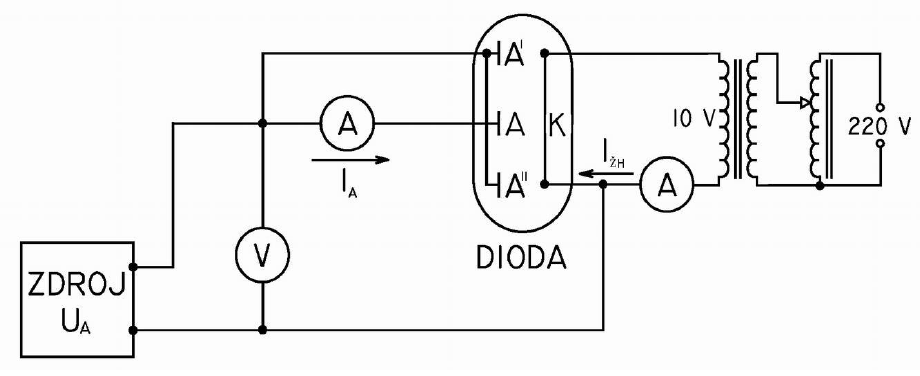
\includegraphics[width=12cm]{att/pyromet2.png}
%			\caption{Zapojení pro měření náběhového proudu. Převzato z \cite{bib:zadani}.}
%			\label{fig:s_aparatura_nasyc}
%			\end{figure}	
%			
%			\begin{figure}[h!]
%			\centering
%			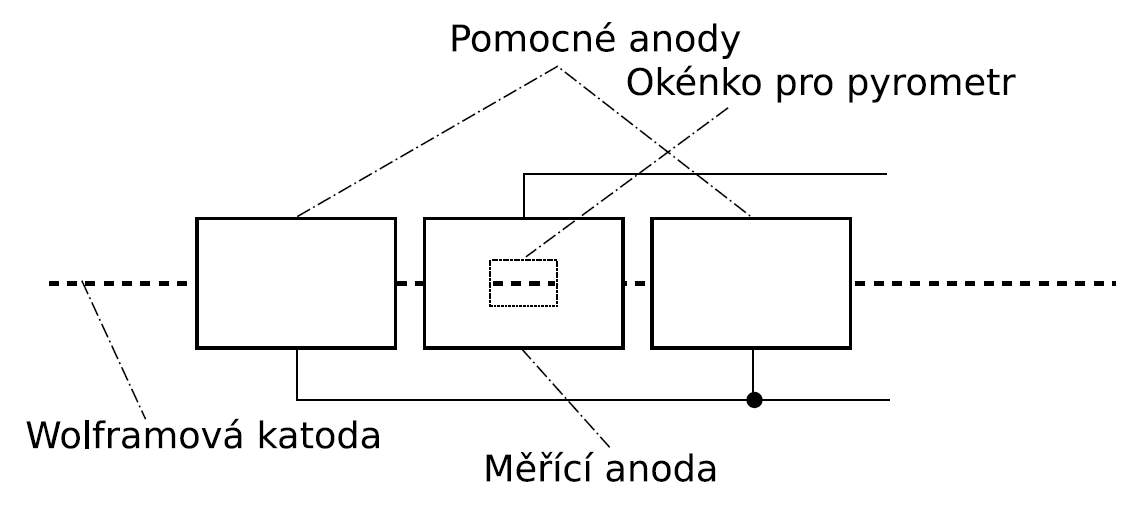
\includegraphics[width=10cm]{att/pyromet.png}
%			\caption{Geometrie uspořádání vakuové diody s pomocnými anodami pro dosažení homogenního pole. \newline Převzato z \cite{bib:zadani}.}
%			\label{fig:s_dida}
%			\end{figure}
%	
\clearpage
\section{Grafy}

	\begin{figure}[h!]
	\begin{center}
	    \vspace*{-1cm}
		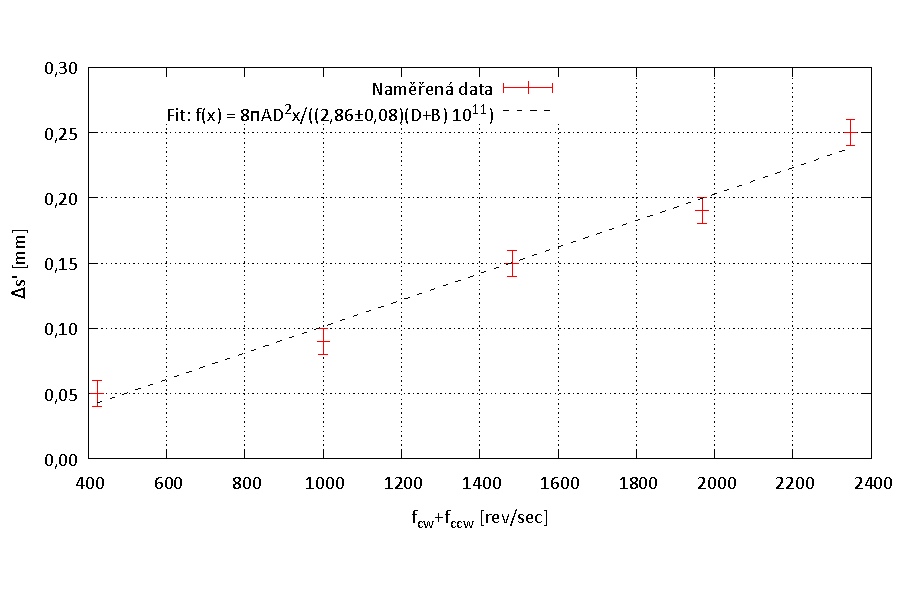
\includegraphics[width=\linewidth]{../gnuplot/c.pdf}
	    \vspace*{-2cm}
		\caption{Závislost rozdílu naměřených poloh bodů $\Delta s'$ na součtu frekvencí $f_{cw}$ a $f_{ccw}$. Hodnoty jsou následně proloženy funkcí (\ref{eq:fit}), ze které je určen parametr $c$ (rychlost světla). }
		\label{fig:g_data}
	\end{center}
	\end{figure}
	
%\clearpage

					
%\clearpage
% --- Konec dokumentu --------------------------------------------------


\end{document}

